\documentclass[12pt]{article}  % standard LaTeX, 12 point type
\usepackage{amsfonts,latexsym}
\usepackage{amsthm}
\usepackage{amssymb}
\usepackage[utf8x]{inputenc} % Кодировка
\usepackage[english]{babel} % Многоязычность
\usepackage{amsmath}
\usepackage{tikz}
\usetikzlibrary{automata,positioning}

\usepackage{algpseudocode}
\usepackage{algorithm}
\usepackage{caption}
\usepackage{algorithmicx}


\newtheorem{theorem}{Theorem}[section]
\newtheorem{proposition}[theorem]{Proposition}
\newtheorem{lemma}[theorem]{Lemma}
\newtheorem{corollary}[theorem]{Corollary}
\newtheorem{conjecture}[theorem]{Conjecture}

\theoremstyle{definition}
\newtheorem{definition}{Определение}[section]
\newtheorem{example}{Example}[section]

% unnumbered environments:

\theoremstyle{remark}
\newtheorem*{remark}{Remark}
\newtheorem*{notation}{Notation}
\newtheorem*{note}{Note}

\setlength{\parskip}{5pt plus 2pt minus 1pt}
%\setlength{\parindent}{0pt}

\usepackage{color}
\usepackage{listings}
\usepackage{caption}
\usepackage{graphicx}
\usepackage{ucs}

\newcommand{\tab}[1][0.3cm]{\ensuremath{\hspace*{#1}}}
% A generalized view on parsing and translation
% http://dl.acm.org/citation.cfm?id=2206331
\title{Arbirary CFPQ to Dyck language constrained querying}
% Context-free path querying ...
\author{Semyon Grigorev
\\
       {Saint Petersburg State University}\\
       {7/9 Universitetskaya nab.}\\
       {St. Petersburg, 199034, Russia}\\
       semen.grigorev@jetbrains.com, rsdpisuy@gmail.com
       }
\date{}

\begin{document}

\algtext*{EndWhile}% Remove "end while" text
\algtext*{EndIf}% Remove "end if" text
\algtext*{EndFor}% Remove "end for" text
\algtext*{EndFunction}% Remove "end function" text

\maketitle

This reduction is inspired by the construction described in~\cite{OptimalDLR}.

Consider a context-free grammar $\mathcal{G}=(\Sigma, N, P, S)$ in BNF where $\Sigma$ is a terminal alphabet, $N$ is 
a nonterminal alphabet, $P$ is a set of productions, $S \in N$ is a start nonterminal.
Also we denote a directed labeled graph by $G=(V,E,L)$ where $E \subseteq V \times L \times V$ and $L \subseteq \Sigma$. 

We should construct new input graph $G'$ and new grammar $\mathcal{G'}$ such that $\mathcal{G'}$ specifies a Dyck language and there is a simple mapping from $\text{CFPQ}(\mathcal{G'}, G')$ to $\text{CFPQ}(\mathcal{G}, G)$.
Step-by-step example with description is provided below.
 
Let the input grammar is 
\begin{align*}
S & \rightarrow a \ S \ b \ | \ a \ C \ b 
\\
C & \rightarrow c \ | \ C \ c
\end{align*}

Let the input graph is
\\
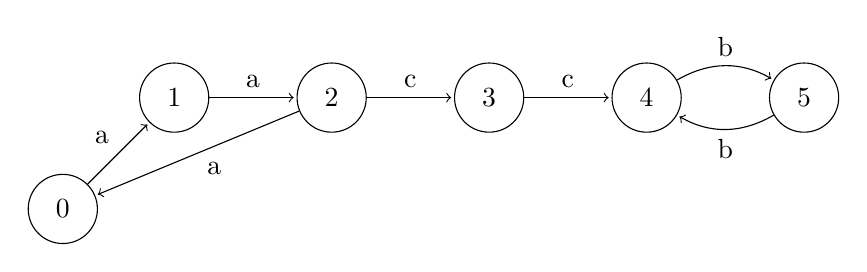
\begin{tikzpicture}[shorten >=1pt,node distance=2cm,on grid,auto] 
   \node[state] (q_0)   {$0$}; 
   \node[state] (q_1) [above right=of q_0] {$1$}; 
   \node[state] (q_2) [right=of q_1] {$2$}; 
   \node[state] (q_3) [right=of q_2] {$3$};
   \node[state] (q_4) [right=of q_3] {$4$};
   \node[state] (q_5) [right=of q_4] {$5$};
    \path[->] 
    (q_0) edge  node {a} (q_1)          
    (q_1) edge  node {a} (q_2)
    (q_2) edge  node {a} (q_0)
    (q_2) edge  node {c} (q_3)
    (q_3) edge  node {c} (q_4)
    (q_4) edge[bend left, above]  node {b} (q_5)
    (q_5) edge[bend left, below]  node {b} (q_4);
\end{tikzpicture}

\begin{enumerate}
\item Let $\Sigma_{()} =\{ t_( , t_)  | t \in \Sigma \}$.
\item Let $N_{()} = \{ N_( , N_) | N \in N  \}$.
\item Let $M_{\mathcal{G}} = (V_{\mathcal{G}}, E_{\mathcal{G}}, L_{\mathcal{G}})$ is a directed 
labeled graph, where $L_{\mathcal{G}} \subseteq (\Sigma_{()} \cup N_{()})$.
This graph is created the same manner as described in~\cite{OptimalDLR} but we do not require the grammar be in CNF.
Let $x \in V_{\mathcal{G}}$ and $y \in V_{\mathcal{G}}$ is ``start'' and ``final'' vertices respectively. 
This graph may be treated as a finite automaton, so it can be minimized and we can compute an $\varepsilon$-closure if the input grammar contains $\varepsilon$ productions.
The graph $M_{\mathcal{G}}$ for our example is:
\\
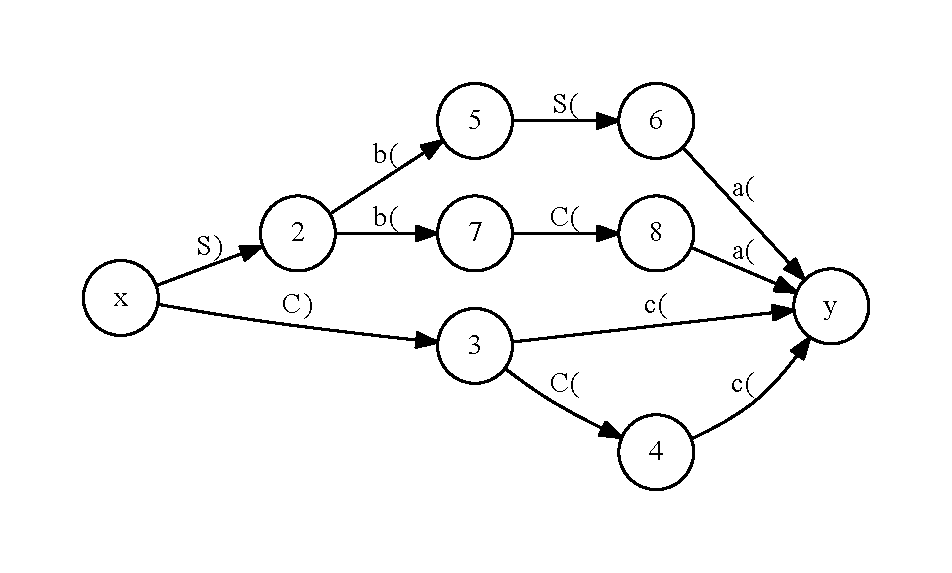
\includegraphics[width=.7\textwidth]{dot/grammar_1.pdf}


The minimized graph:
\\
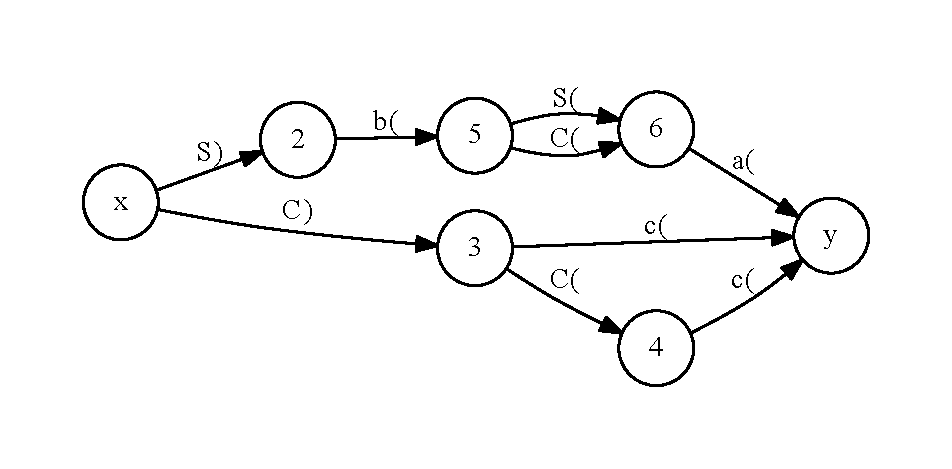
\includegraphics[width=.7\textwidth]{dot/grammar_min.pdf}


\item For each $v \in V$ create $M_{\mathcal{G}}^v$: unique instance of $M_{\mathcal{G}}$.
\item New graph $G^{'}$ is a graph $G$ where each label $t$ is replaced with $t_{)}^i$ and some additional edges are created:
\begin{itemize}
\item Add an edge $(v', S_(, v)$ for each $v \in V$. 
\item And the respective $M_{\mathcal{G}}^v$ for each $v \in V$:
  \begin{itemize}
    \item reattach all edges outgoing from $x^v$ (``start'' vertex of $M_{\mathcal{G}}^v$) to $v$;
    \item reattach all edges incoming to $y^v$ (``final'' vertex of $M_{\mathcal{G}}^v$) to $v$.    
  \end{itemize}
  New input graph is ready:
  
  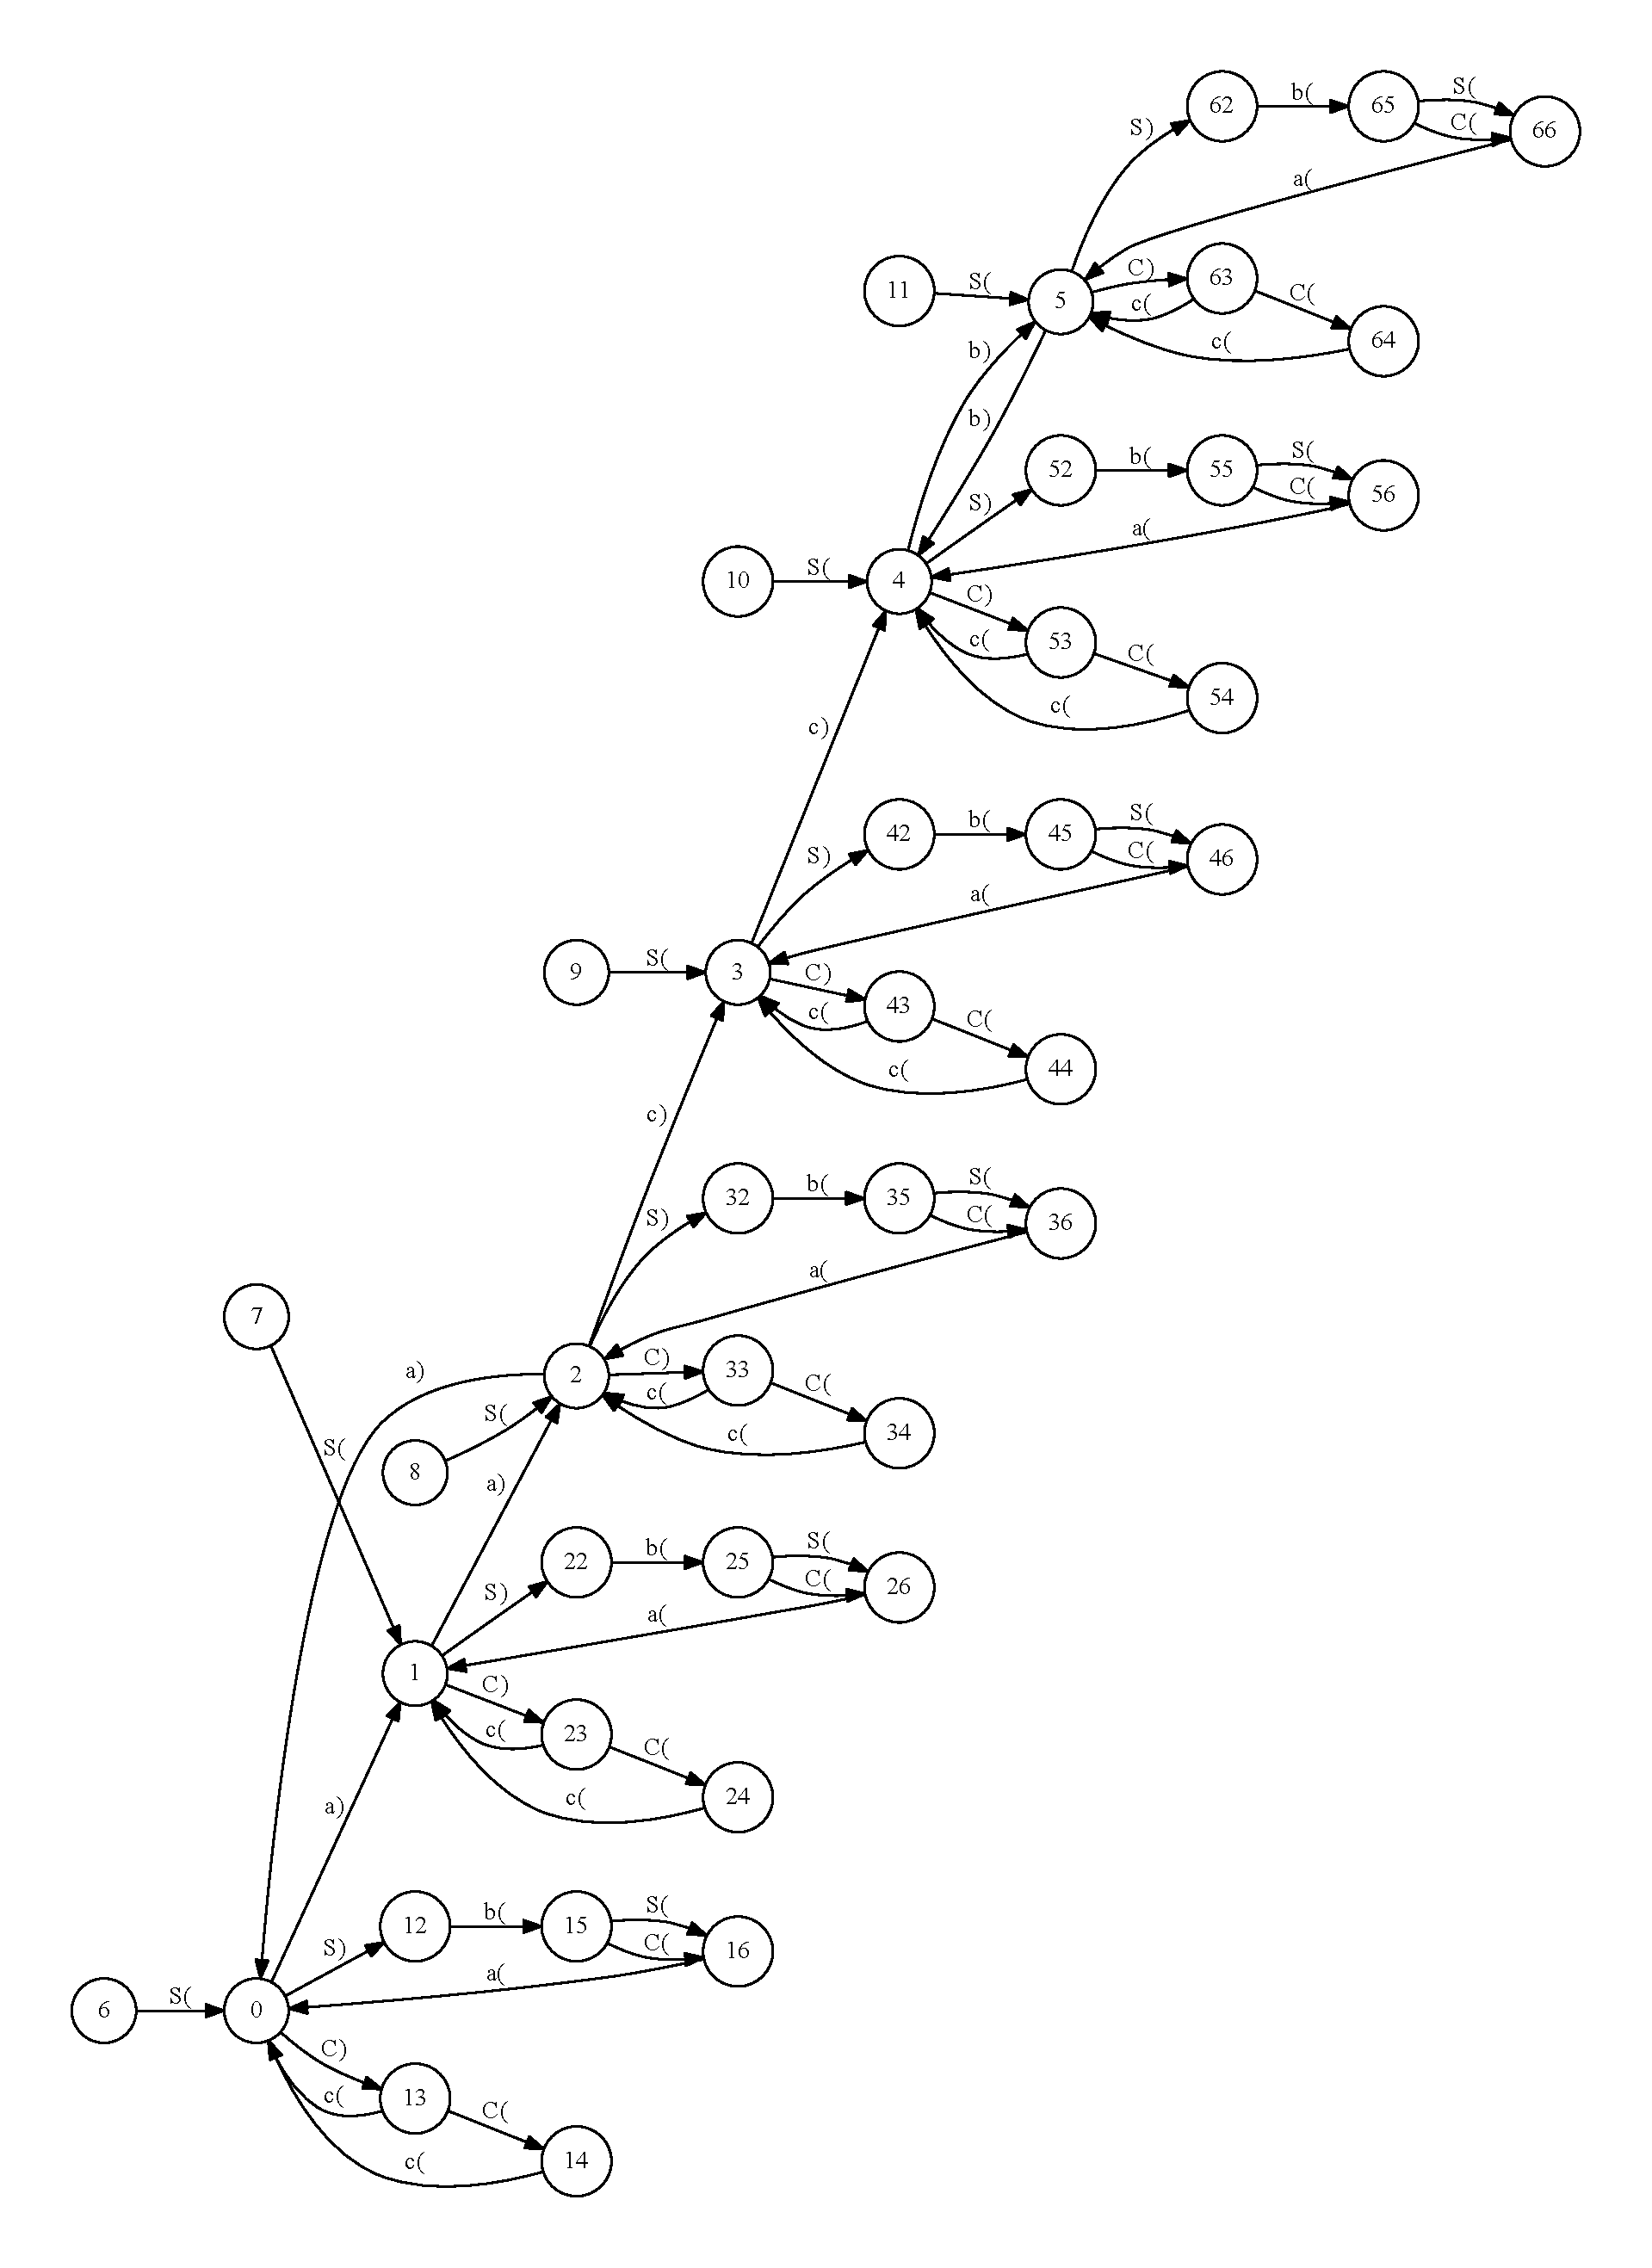
\includegraphics[width=.9\textwidth]{dot/input_new_min.pdf}
\end{itemize}

\item New grammar $\mathcal{G'}=(\Sigma^{'}, N', P', S')$ where $\Sigma^{'} = \Sigma_{()} \cup N_{()}$, $N' = \{ S' \}$, $P' = \{ S' \rightarrow b_( \ S' \ b_); S' \rightarrow b_( \ b_) \ | \ b_(, b_{)} \in \Sigma^{'} \} \cup \{ S' \rightarrow S' \ S' \}$ is a set of productions, $S' \in N'$ is a start nonterminal.
\end{enumerate}

Now, if $\text{CFPQ}(\mathcal{G'}, G')$ contains a pair $(u'_0, v')$ such that $e=(u'_0, S_( , u'_1) \in E'$ is an extension edge (step 5, first subitem), then  $(u'_1, v') \in \text{CFPQ}(\mathcal{G}, G)$.
In our example, we can find the following path: $7 \xrightarrow{S_(} 1 \xrightarrow{S_)} 22 \xrightarrow{b_(} 25 \xrightarrow{C_(} 26 \xrightarrow{a_(} 1   
\xrightarrow{a_)} 2 \xrightarrow{C_)} 33 \xrightarrow{C_(} 34 \xrightarrow{c_(} 2  \xrightarrow{c_)} 3 \xrightarrow{C_)} 43 \xrightarrow{c_(} 3 \xrightarrow{c_)} 4 \xrightarrow{b_)} 5$. 
Edge $7 \xrightarrow{S_(} 1$ is the extension, so (1,5) should be in $\text{CFPQ}(\mathcal{G}, G)$ and it is true.


\section{Modified algorithm}

\begin{algorithm}[!ht]
\begin{algorithmic}[1]
\caption{Digraph flat exact paths}
\label{parsing}
\Function{Digraph-flat-exact-paths}{$G$}
  \State{$\{{D_k}^{(-1)}, {D_k}^{(0)}, {D_k}^{(+1)} \} \gets$ \Call{Init-Adjacency-Matrices}{$G$}}
  \State{$M_1 \gets$ \Call{AGMY-Code-then-Sum}{${D_1}^{(-1)}, {D_1}^{(0)}, {D_1}^{(+1)}$}}
  \State{$\dots$}
  \State{$M_k \gets$ \Call{AGMY-Code-then-Sum}{${D_k}^{(-1)}, {D_k}^{(0)}, {D_k}^{(+1)}$}}
  \State{$n \gets |V|$}
  \For{$l \in [2 \dots \lceil \text{log} \ n \rceil + 1]$} \Comment{Upper bound should be analized carefully}
     \State{$M' \gets $ \Call{Markup-Minus-One-Edges}{$M_1$}} \Comment{AGMY, mark $-1$ edges}     
     \State{$M_1 \gets M' \times M_1$}  \Comment{AGMY, non-Dyck 0 edges are detectable}
     \State{$\dots$} \Comment{Do for all $M_i$}
     \State{$M_k \gets M_k \times M_k$}
     \State{Remove $\pm 1$ edges from all $M_i$}
     \State{$M_1 \gets$ \Call{Normalize-and-Divide-by-2}{$M_1$}}
     \State{$\dots$}
     \State{$M_k \gets$ \Call{Normalize-and-Divide-by-2}{$M_k$}}
     \State{$Z \gets$ \Call{Get-Zero-Edges}{$M_1$}}
     \State{$Z \gets Z + $ \Call{Get-Zero-Edges}{$M_2$}}
     \State{$\dots$}
     \State{$Z \gets Z + $ \Call{Get-Zero-Edges}{$M_k$}}
     \State{$M_1 \gets Z \times M_1 \times Z$}  \Comment{AGMY, extend $\pm 1$  and 0 edges for all $M_i$}
     \State{$\dots$}
     \State{$M_k \gets Z \times M_k \times Z$}
  \EndFor
\EndFunction
\end{algorithmic}
\end{algorithm}


\begin{thebibliography}{9}

\bibitem{OptimalDLR}
Krishnendu Chatterjee, Bhavya Choudhary, and Andreas Pavlogiannis. 
2017. 
\emph{Optimal Dyck reachability for data-dependence and alias analysis.}
Proc. ACM Program. Lang. 2, POPL, Article 30 (December 2017), 30 pages. DOI: 
https://doi.org/10.1145/3158118


%\bibitem{ParsingWithPictures}
%  Keshav Pingali, and Gianfranco Bilardi. 
%  \emph{A Graphical Model for Context-Free Grammar Parsing.}
%   International Conference on Compiler Construction. Springer, Berlin, Heidelberg, 2015.


\end{thebibliography}


\end{document}